\section{Datenbank}
\subsection{Definition}
Eine Datenbank ist eine große Sammlung von strukturierten und organisierten Daten,
die in einem Computersystem gespeichert sind. Gesteuert wird eine solche Datenbank von
einem \textbf{Datenbankmanagementsystem (DBMS)}. Die Daten und das DBMS werden zusammen als
Datenbanksystem bezeichnet, jedoch meistens als Datenbank abgekürzt.

Die Daten in den gängigsten verwendeten Datenbanken werden in Zeilen und Spalten unterteilt und
in einer Tabelle modelliert. Aufgrund dieser Struktur können diese Daten dann einfach, abgerufen,
modifiziert, aktualisiert, kontrolliert und organisiert werden. Fast alle Datenbanken verwenden
zum Abfragen oder Schreiben von die \textit{Structured Query Language (SQL)}.
\cite{Datenbank}

\subsection{Datenbankmanagementsystem}
Als \textit{Datenbankmanagementsystem(DBMS)} wird eine Datenbankprogramm bezeichnet die als Schnittstelle
zwischen Usern und der Datenbank dient. Es ermöglicht den Benutzern
Informationen aufzurufen zu aktualisieren oder zu optimieren. Administrative Aufgaben
werden durch so ein \textit{DBMS} ebenso erleichtert. Abläufe wie Leistungsüberwachung,
Abstimmung sowie Backup und Wiederherstellung werden ermöglicht.

Die wohl bekanntesten \textit{DBMSs} sind:

\begin{itemize}
    \item  MySQL
    \item Microsoft Access
    \item Microsoft SQL Server
    \item File Maker Pro
    \item Oracle database
    \item dBase
\end{itemize}

\subsection{Structured Query Language (SQL)}
Die Programmiersprache SQL wird heutzutage von fast allen relationalen Datenbanken verwendet
um Daten Abzufragen, Manipulieren und zu Definieren. SQL hat außerdem zu vielen Erweiterungen
bei großen Unternehmen wie IBM, Oracle und Microsoft.

\subsection{MySQL}

\textit{MYSQL} ist ein relationales Datenbankmanagementsystem, das auf dem Open-Source
Programmiersprache \textit{SQL} basiert. Eingeführt wurde es 1995 vom schwedischen Unternehmen
\textit{MySQLAB} und wurde dann im Jahre 2010 von \textit{Oracle} übernommen. Der Name fügt sich
aus der Kombination "My", der Name einer Tochter eines Mitbegründers und ``SQL'' der Abkürzung
für Structured Query Language zusammen.

Um das Prinzip von \textit{MYSQL} zu verstehen muss man zwei Konzepte verstehen.

\subsubsection{Relationale Datenbanken}
Bei Relationalen Datenbanken werden die Daten in Form von Tabellen dargestellt, anstelle von
einem großen Speicherbereich.
Bei relativen Datenbanken gibt es einen sogenannten \textbf{Schlüssel}. Mithilfe diesen Schlüssels
ist es möglich, Daten zwischen verschiedenen Tabellen miteinander zu verknüpfen. In der Regel ist
ein solcher Schlüssel eine \textbf{eindeutige Identifikationsnummer (ID)}.
\subsubsection{Client-Server-Model}
\textit{MySql} basiert außerdem auf dem Prinzip des \textbf{Client-Server-Model}. Im \textbf{Server}
befinden sich die Daten und um auf diese zugreifen zu können wird ein sogenannter \textbf{Client}
benötigt. Unter \textit{SQL} sendet also der Client eine Anfrage auch genannt \textbf{resquest}
worauf der Datenbankserver mit den benötigten Daten antwortet \textbf{response} .

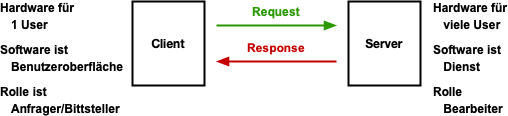
\includegraphics[width=0.75\textwidth]{Backend/ClientSever.png}

\subsection{Andere Datenbanktypen}
Wie bereits oben beschrieben ist \textit{MySql} ein relatives Datenbanksystem. Es gibt
jedoch einige weiter Datenbanktypen.

\subsubsection{Objektorientierte Datenbanken}
Die Informationen werden in einer objektorientierten in Form von Objekten dargestellt.

\subsubsection{Verteilte Datenbanken}
In einer verteilten Datenbank werden die Informationen in zwei oder mehreren Dateien gespeichert.
Diese Dateien können auf mehreren Rechnern verteilt sein, die entweder an einem einzigen Standort
sind oder welche über ein Netzwerk miteinander kommunizieren.

\subsection{Data Warehouse}
Data Warehouse Datenbanken bestehen aus einem zentralen Daten Repository. Es wurde speziell für
schnelle Anfragen und Analysen konzipiert.

\subsection{NoSQL-Datenbanken}
Im Gegensatz zu einem relativen Datenbanksystem ermöglicht eine \textit{NoSql} Datenbank,
semistrukturierter Daten bzw. unstrukturierte Daten zu speichern und verändern. NoSql Datenbanken
setzten zur Organisation nicht auf sogenannte \textbf{keys}, sondern auf Wertepaare, Objekte, Dokumente,
Listen oder Reihen. Da \textit{NoSql} Systeme sehr flexibel sind, eignen sie sich
besonders für große Datenmengen sogenannte \textbf{Big Data}. Die bekanntesten
\textit{NoSql} Datenbanksysteme sind
\begin{itemize}
    \item Apache
    \item Cassandra
    \item Riak
    \item MongoDB
    \item Redis
    \item CouchDB
\end{itemize}

\subsection{Diagrammdatenbanken}
Daten werden anhand von Entitäten und ihren Beziehungen abgespeichert.

\subsection{OLTP-Datenbanken}
Eine \textit{OLTP} Datenbank kennzeichnet sich dadurch, dass sie schnell analytisch und für eine
Vielzahl von Transaktionen mehrerer Benutzer ausgelegt ist.

Das sind natürlich nicht alle vorhandenen Datenbanktypen. Die Anderen sind jedoch
nicht weit verbreitet und speziell für wissenschaftliche, finanzielle oder andere Funktionen konzipiert.


\cite{MySQL}
\label{db}

